% vim: set textwidth=78 autoindent:

\subsection{Extension de texte Délimité}\label{label_dltext}    

% when the revision of a section has been finalized, 
% comment out the following line:
%\updatedisclaimer

%The Delimited Text plugin allows you to load a delimited text file as a layer in QGIS.
L'extension Fichier texte délimité permet de charger un fichier texte délimité comme couche dans QGIS.

%\minisec{Requirements}
\minisec{Exigences}

%To view a delimited text file as layer, the text file must contain:
Pour afficher un fichier texte délimité comme couche, le fichier texte doit contenir :

% \begin{enumerate}      
% \item A delimited header row of field names. This must be the first line in the text file.
% \item The header row must contain an X and Y field. These fields can have any name.
% \item The x and y coordinates must be specified as a number. The coordinate system is not important.
% \end{enumerate}
\begin{enumerate}      
\item Une ligne d'entête délimitée avec les noms de champs. Cette ligne doit être la première du fichier texte.
\item La ligne d'entête doit contenir des champs X et Y. Ces champs peuvent avoir n'importe quel nom.
\item Les coordonnées X et Y doivent être de type numérique. Le système de coordonnées n'est pas important.
\end{enumerate}

%As an example of a valid text file we import the elevation point data file 
%\filename{elevp.csv} coming with the QGIS sample dataset (See Section~\ref{label_sampledata}):
Comme exemple de fichier texte valide, nous pouvons importer le fichier de points d'élévation
\filename{elevp.csv} fourni avec le jeu de données échantillon de QGIS (Voir Section~\ref{label_sampledata}) :

\begin{verbatim} 
X;Y;ELEV
-300120;7689960;13
-654360;7562040;52
1640;7512840;3
[...]
\end{verbatim}

% Some items of note about the text file are:
On notera les points suivants à propos du fichier texte :

% \begin{enumerate}
% \item The example text file uses \mbox{$;$} as delimiter. Any character can be used to delimit the fields.
% \item The first row is the header row. It contains the fields X, Y and ELEV.
% \item No quotes ({\tt{}"{}}) are used to delimit text fields.
% \item The x coordinates are contained in the {\em X} field.
% \item The y coordinates are contained in the {\em Y} field.
% \end{enumerate}
\begin{enumerate}
\item Le fichier texte d'exemple utilise \mbox{$;$} comme délimiteur. N'importe quel caractère peut être utilisé pour délimiter les champs.
\item La première ligne est la ligne d'entête. Elle contient les champs X, Y et ELEV.
\item Les guillemets ({\tt{}"{}}) ne peuvent pas être utilisés pour délimiter les champs de texte.
\item les coordonnées x sont inclues dans le champ {\em X}.
\item les coordonnées y sont inclues dans le champ {\em Y}.
\end{enumerate}

% \minisec{Using the Plugin}
% To use the plugin you must have QGIS running and use the Plugin Manager to load the plugin:
\minisec{Utilisation de l'extension}
Pour utiliser l'extension, QGIS doit être lancé. Utilisez le Gestionnaire d'extensions pour charger l'extension : 

% Start QGIS, then open the Plugin Manager by choosing \mainmenuopt{Plugins} > \dropmenuopttwo{mActionShowPluginManager}{Plugin Manager...}
Démarrez QGIS, puis ouvrez le gestionnaire d'extensions en cliquant sur \mainmenuopt{Extensions} > \dropmenuopttwo{mActionShowPluginManager}{Gestionnaire d'extensions...}

% \index{plugins!manager}
% The Plugin Manager displays a list of available plugins.
% Those that are already loaded have a check mark to the left of their name.
% Click on the checkbox to the left of the \checkbox{Add Delimited Text Layer} plugin and click \button{OK} to load it as described in Section \ref{sec:managing_plugins}.
\index{extensions!gestionnaire}
Le gestionnaire d'extension affiche une liste des extensions disponibles.
Celles qui sont déjà chargées sont cochées en début de ligne.
Cochez la case de l'extension \checkbox{Add Delimited Text Layer} et cliquez sur \button{OK} pour charger l'extension comme indiqué dans la Section \ref{sec:managing_plugins}.

% Click the new toolbar icon \toolbtntwo{delimited_text}{Add Delimited Text Layer} to open the Delimited Text dialog as shown in Figure
% \ref{fig:delim_text_plugin_dialog}.
Cliquez sur la nouvelle icône de la barre d'outils \toolbtntwo{delimited_text}{Ajoutez un fichier texte délimité} pour ouvrir la boîte de dialogue Texte Délimité comme indiqué dans la Figure 
\ref{fig:delim_text_plugin_dialog}.

\begin{figure}[ht]
   \begin{center}
   \caption{Delimited Text Dialog \nixcaption}\label{fig:delim_text_plugin_dialog}\smallskip
   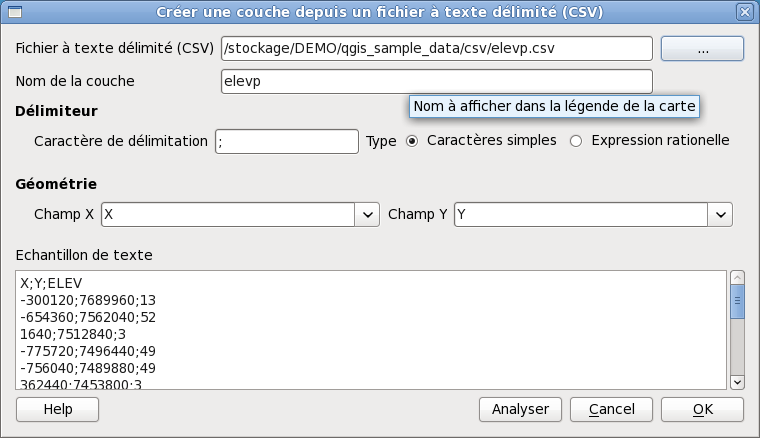
\includegraphics[clip=true, width=14cm]{delimited_text_dialog}
   \end{center}  
\end{figure}

% First select the file \filename{qgis\_sample\_data/csv/elevp.csv} to import by clicking 
% on the \button{Browse} button. Once the file is selected, the plugin attempts to parse the file 
% using the last used delimiter, in this case \mbox{$;$}. To properly parse the file, it 
% is important to select the correct delimiter. To change the delimiter to tab use 
% \mbox{$\backslash$}t (this is a regular expression for the tab character).
% After changing the delimiter, click \button{Parse}.
Sélectionnez d'abord le fichier \filename{qgis\_sample\_data/csv/elevp.csv} à importer en cliquant
sur le bouton \button{Browse}. Une fois que le fichier est sélectionné, l'extension va tenter d'analyser le fichier
en utilisant le dernier délimiteur utilisé, en l'occurrence \mbox{$;$}. Pour analyser correctement le fichier, il 
est important de sélectionner le bon délimiteur. Pour changer le délimiteur en tab, 
utilisez \mbox{$\backslash$}t (expression habituelle du caractère tab).
Après avoir changé le délimiteur, Cliquez sur \button{analyser}.

% Choose the X and Y fields from the drop down boxes and enter a Layer name \filename{elevp} 
% as shown in Figure \ref{fig:delim_text_plugin_dialog}. To add the layer to the map, click 
% \button{Add Layer}. The delimited text file now behaves as any other map layer in QGIS.
Choisissez les champs X et Y depuis les listes déroulantes et entrez un nom de couche (par exemple \filename{elevp}) comme indiqué dans la Figure \ref{fig:delim_text_plugin_dialog}. Pour ajouter la couche à la carte, cliquez sur \button{Add Layer}. Le fichier texte délimité se comporte maintenant comme n'importe quel autre calque dans QGIS.

